

\documentclass[titlepage, 12pt]{article}
\usepackage{lipsum}
\usepackage{amsmath}
\usepackage{amssymb}
\usepackage{amsthm}
\usepackage{color}
\usepackage{graphicx}
\usepackage{mnsymbol}
\usepackage{enumerate}
\setlength{\textwidth}{5.5in}
\setlength{\textheight}{8in}
\newcommand{\h}[1]{\colorbox{yellow}{#1}}
\newcommand{\problem}{\subsection*}
\newcommand{\R}{\mathbb{R}}
\newcommand{\F}{\mathbb{F}}
\newcommand{\Z}{\mathbb{Z}}
\newcommand{\Q}{\mathbb{Q}}
\newcommand{\C}{\mathbb{C}}

\begin{document}
\title{{\bf AI Database in the Prometheus Architecture}}
 
\vspace{5 mm} 
\author{
          \text{S}\text{an}\tex{t}\text{ia}\text{go }\text{P}\text{aiv}a \\\\
               \text{C}\text{OMP} 396 - Undergraduate Research Project
          }
\date{Date Submitted: September 4, 2013}

\maketitle

\pagenumbering{gobble}
\clearpage
\thispagestyle{empty}
%----------------------------------------------------------------------------------------
%	ABSTRACT
%----------------------------------------------------------------------------------------

%\begin{center}
\section*{Abstract}
%\end{center}
\noindent The Prometheus project is an ongoing project at McGill University that aims to create a fully intelligent brain similar to our own by simulating lower life forms such as ants and gradually working towards fully autonomous robots. This project uses the Prometheus architecture to expand the functionality of the AI brain by implementing a database component using XML files, adding a large amount of information into the database, and then testing this system for its efficiency and correctness.

%----------------------------------------------------------------------------------------
%	ACKNOWLEDGEMENTS	
%----------------------------------------------------------------------------------------

%\begin{center}
\section*{Acknowledgements}
%\end{center}
\noindent I want to thank Prof. Vybihal for his time, support, and mentoring through this project. I gained a lot of experience under his supervision and I would like to acknowledge him for continually fostering creativity in exploring the potential of Artificial Intelligence. Thank you.  I would also like to thank the numerous groups that created and worked on the Prometheus Project for their contribution to this ongoing endeavor.

\newpage
\tableofcontents
\newpage
\clearpage
\pagenumbering{arabic}

%----------------------------------------------------------------------------------------
%	ARTICLE CONTENTS
%----------------------------------------------------------------------------------------

\section{Introduction} 

Prometheus is an ongoing project at McGill University under the supervision of Prof. Joseph Vybihal. The project is a playground for artificial intelligence concepts, it creates a 3D world in which virtual ants can evolve and interact. \\

The current version of Prometheus uses ants in a simulated world that are guided mostly by smells and attempt to simulate the effects of learning, reasoning, and decision-making. This version is composed of five main modules: the Simulator, the AI module, the World, and two interfaces that interact with simulations. The main focus of this project is on the AI module which is divided into four main components: the Neural Network, the Knowledge Node, the Expert System, and the Meta-Modeller. \\

\subsection{Project goals}

The desired goal of this project was to develop a database-like system that would interface the ant world simulator with the four AI modules of the ant's brain. This database contains both DNA information of the simulated ant as well as a collection of previously learned experiences and actions taken. \\

This database provides a framework to create different ants with similar learning opportunities, but different capabilities. Hence, it provides a setting to test and work with different ant avatars. The current version of this system implements XML files to store and retrieve this information, however it has not been tested and implemented by the AI modules yet. \\

In addition, another focus of the project was to develop a better model of smell, being a single object and equal to all ants, with a new model that resembles reality. The ants have the ability to smell and to diffuse a smell; each have a specific implication and a different duration according to its purpose.  

\section{Background Information}

\subsection{The Prometheus Brain Model}

The Prometheus project is abstraction of the mind. There are four levels of the brain, each level accomplishing a specific task. \\

\begin{center}
{\bf Project Architecture} 
\end{center}

\begin{figure}[h!]
    \centering
    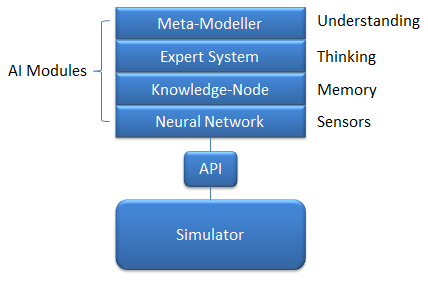
\includegraphics{aimodules.png}
\caption{Prometheus Project Architecture}
\end{figure}

We now provide a small description of each AI module. 

\begin{itemize}
\item {\bf The Neural Network Module} \\
The Neural Network processes the signals from the outside world (the Simulator). These signals reach the module through a sensor that convert signals into discrete units and sends it as input to the Neural Network. The Neural Network then produces predicate calculus strings which in turn are used as input to the knowledge node to initiate the memory retrieval process. This neural network is currently implemented as a Perceptron, but it is currently transitioning towards a Knowledge-Base Cascade-Correlation (KBCC) Neural Network. 

\item {\bf The Knowledge-Node Module} \\
The Knowledge-Node takes the output information from the Neural Network to use it as part of the ant AI's memory. For example, the AI's memory include memorising visual landmarks and using these memories for navigation during foraging.  

\item {\bf The Expert System Module} \\
The output of the Knowledge-Node is fed into the Expert System. At this time, the Expert System is a production system that reasons on the input it receives from the Knowledge-Node. The Expert System can perform complex decisions compared to the Neural Network. It should provide a recommendation on what should be done next. 

\item {\bf The Meta-Modeller Module} \\
The Mata-Modeller is currently under development and it decides if it accepts the recommendation or not. If it accepts the recommendation, then its model of the ant's goals and intentions is updated. 
\end{itemize}


\subsection{Ant morphology}
Ants have three main parts of the body: the head, metasoma (the ``thorax"), and the gaster (the ``abdomen").  They sense things with their two long antennae connected to their head. These antennae are used to detect flavors, sounds and odors.  It can also be used to communicate with other ant. Ants also have two front eyes that can see very short distances; some ants have an eye located on the top of their head to sense sun light [2]. \\

Furthermore, ants have jaws called mandibles which are used to pick up pieces of food, to dig nests, and as weapons for fighting. The thorax contains the three pairs of legs.  Each leg has two tiny legs on the end which helps the ant crawl upside down.  \\

\subsection{Types of ants}
Ants work together in a colony as a super-organism. Hence, there are determined functions that ants have to accomplish. In this project, there are, basically, five types of ants: the Queen, the Worker, the Soldier, the Hunter, and the Male. [5] Here is a basic description of each type: 

\begin{itemize}
\item Queen: the mother of all ants in a colony, solely responsible for reproduction 
\item Worker: Ants responsible for construction, transportation, and various labor works in a colony 
\item Soldier: Ants responsible for the security and defence in a colony
\item Hunter: Ants responsible for food gathering
\item Male: Ant responsible to mate with the Queen
\end{itemize}

The Queen, Soldiers, Workers, Hunters ants are all female. The Male ant is the only male. [5]

\subsection{Foraging, Pheromones, and External Factors}
Foraging in ants involves exploration and search in surrounding  area for food source and exploitation of a found food source effectively. This based on the concept of ``pheromone" and trail following. \\

There are two main procedures all species of ants roughly follow when foraging: secreting pheromones during exploration and hence creating ``pheromone trails", following which at later stages are used as a navigation mechanism and memorization and recalling of landmarks seen on a path that eventually led to a food source. [4]\\

Ants release a chemical substance called ``Pheromome" on the ground when it encounters danger or to show fellow ants the shortest path to food.  There are external factors that influence the intensity of the smell such as humidity, water and winds. In other words, every pheromone released on the ground has a decay rate which can be reinforced by ants if important. More detail will be provided in Section 4 of this report. 

\section{The AI Database}

\subsection{Overview}
The AI Database aims to provide a framework where we can represent different types of ants and switch on and off different characteristics, parameters, and methods according to our needs. The information is stored in a XML file to be accessed by higher levels of the brain when it comes to take a decision. \\

In this section, we will talk about the design and implementation of this database. Then, we will describe how is the process of storing and retrieving information works with three arrays: the Gene array, the Expression array, and the Truevals array. We will describe their functionality and overall impact in the project. \\

\subsection{Design}

A general XML file database is composed of two main parts: the Body Elements and the AI Elements. The most important part of this design is its modularity and its the ability to generate various ants avatars by changing parameter values and attributes. \\

We will now provide a short description of the database elements.  

\begin{itemize}
\item {\bf Body Elements $<$body$>$}\\
It is composed of two pieces of information: the genes and the expressions. The genes represent the general DNA-like information of the ant. The expressions are attributes that give value to given genes. For example, a gene could be the ant's strength and the expression value could be an given number that represents the strength of the ant. 

\item {\bf AI Elements $<$AI$>$}\\
It is composed of four pieces of information: the Meta-Modeller, the K-Expert System, the Knowledge-Node, and the Neural Network. Each AI module will store and retrieve information inside each of these modules for a particular ant avatar. \\

As a result, we will have ant avatars with similar learning abilities, but different capabilities. For instance, a blind ant will have different training sets than a regular ant, and therefore the ant might take different decisions because it is exposed to a different environment. In this point, the AI elements are not implemented and are therefore non-functional. 
\end{itemize}

\newpage

\begin{figure}[h!]
    \centering
    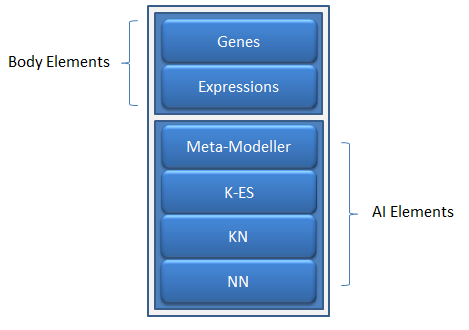
\includegraphics{databasedesign.png}
    \caption{AI database chart}
\end{figure}

\subsection{Implementation}

To implement the database, we wrote two java methods. The first one is called {\tt writeAntXML()} and is located in the XMLGenerator.java class. This method generates a general XML file by prompting the user to enter the ID, the genes, and the expression values for a particular ant. This information is stored in XML file with the particular ant ID. \\

The second one is {\tt readAntBody()} and is located on the XMLReader.java class. This method reads the information stored in the XML file and feds this information into two array lists: the {\tt geneArray} and the {\tt expressionArray}. See Figure 3: Abstraction of the AI Database\\

\newpage

\begin{figure}[h!]
    \centering
    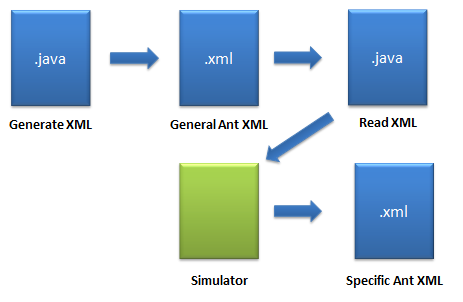
\includegraphics{flowchart.png}
    \caption{Abstraction of the AI Database}
\end{figure}

In the first part of the project, the focus was placed on the first three files: Generate XML, General Ant XML, and Read XML. In the second part, currently under development, we are working on the bottom part of the chart: the Simulator and the Specific Ant XML.\\

In the next page, we provide XML structure format of the General Ant XML file. The General Ant XML file generated by {\tt writeAntXML()} has the following structure: \\

See Figure 4 \\
\newpage
\begin{figure}[h!]
    \centering
    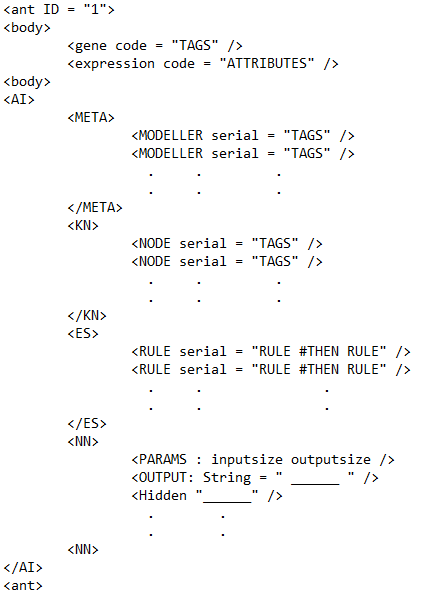
\includegraphics{xml.png}
    \caption{XML structure format.}
\end{figure}

\noindent Notes: 
\begin{enumerate}
\item The TAGS are specific to each module. For the gene element, the TAGS are T/F or Max/Min tags. ATTRIBUTES can be T/F, Max/Min, or integer values
\item AI elements have specific tags relevant to their implementation. For instance, TAGS in the AI elements can be ACT (Activation), THR (Threshold), and AGE (Age). In some cases, TAGS could refer to some predicate calculus operation
\item Each node (NODE), rule (RULE), and modeller (MODELLER) are serialized
\item The Neural Network will have special elements to implement a Knowledge-Base Cascade-Correlation (KBCC) Neural Network which is currently under development
\end{enumerate}

\subsection{DNA Strings}

Ants are modeled using actual ants' model with different body types: head, metasoma, and gaster. The characteristics of these parts are defined according to the ant's type assigned by the queen through a simplified DNA represented by a string of integers. Certain parameters had to be designed for the genes of a virtual ant. 

\begin{center}
{\bf Ant DNA Structure and Expression Values}
\end{center}

\begin{itemize}
\item  {\bf Type Module}
	\begin{itemize}
	\item Ant type
		\begin{itemize}
		\item Queen  = 4
		\item Soldier = 3
		\item Worker = 2
		\item Hunter = 2
		\item Male = 1
		\end{itemize}
	\end{itemize}
\item {\bf Head Module}
	\begin{itemize}
	\item Head size
		\begin{itemize}
		\item Large  = 3, Medium = 2, Small = 1
		\end{itemize}
	\item Front eye 1 distance
	\item Front eye 2 distance
	\item Top eye distance
	\item Mandible size
		\begin{itemize}
		\item Large  = 3, Medium = 2, Small = 1
		\end{itemize}
	\item Antenna 1 size
		\begin{itemize}
		\item Large  = 3, Medium = 2, Small = 1
		\end{itemize}
	\item Antenna 2 size
		\begin{itemize}
		\item Large  = 3, Medium = 2, Small = 1
		\end{itemize}
	\end{itemize}
\item {\bf Metasoma (Thorax) Module}
	\begin{itemize}
	\item Thorax size
		\begin{itemize}
		\item Large  = 3, Medium = 2, Small = 1
		\end{itemize}
	\item Number of Legs, usually 6
	\end{itemize}
\item {\bf Gaster (Abdomen) Module}
	\begin{itemize}
	\item Abdomen size
		\begin{itemize}
		\item Large  = 3, Medium = 2, Small = 1
		\end{itemize}
	\end{itemize}
\item {\bf Energy Module}
	\begin{itemize}
	\item Health Points
		\begin{itemize}
		\item Queen  = 1000
		\item Soldier = 100
		\item Worker = 20
		\item Hunter = 50
		\item Male = 1
		\end{itemize}
	\item Strength level
		\begin{itemize}
		\item Queen: Weak =  100 
		\item Soldier: Strong = 200
		\item Worker: Weak = 100
		\item Hunter: Medium = 150
		\item Male: Weak = 100
		\end{itemize}
	\item Stamina level
	\end{itemize}
\item {\bf Smell Module}\footnote{This will be further discussed in Section 4.} \newpage
\item {\bf Methods Module}
	\begin{itemize}
	\item Different methods that can be turn on and off\footnote{For instance, if we want to use Semantic Primes, then we would turn on this method.}
	\end{itemize} 
\end{itemize}  

The general DNA string of an ant is composed of a string of 4 integers. A specific DNA string of an ant would be composed of more integers to portray different ant avatars with different capabilities. 

\begin{itemize}
\item 1st integer: Type \{Queen  = 4, Soldier = 3, Worker = 2, Hunter = 2, Male = 1\}
\item 2nd integer: Head size \{Large  = 3, Medium = 2, Small = 1\}
\item 3rd integer: Thorax size \{Large  = 3, Medium = 2, Small = 1\}
\item 4th integer: Abdomen size \{Large  = 3, Medium = 2, Small = 1\}
\end{itemize}

For example an ant with DNA string 1111 is a small male ant with small head, thorax and abdomen size. Another example is 3322 is a medium-size female soldier ant with a large head. 

\subsection{Gene and Expression Arrays}

The {\tt readAntBody()} opens a general ant XML file.  It scans the information inside the {\tt <body>} tags. Then, it stores such information into two different array lists: the {\tt geneArray} and the {\tt expressionArray}.\\

For the gene array, we want to turn on and off modules by using True (T) or False (F). In the expression array, we associate the value of the gene with an integer or a string of integers. \\

To keep things simple, we provide the following abstraction: different gene elements belong to different modules. For instance, the Strength level of the ant is a gene element and it belongs to the Energy module.   \\

See Figure 5: Abstraction of the Gene Array. Gene elements belong to specific DNA modules, and Figure 6: Abstraction for the Expression Array. String refers to a string of integers

\newpage

\begin{center}
{\bf DNA Modules inside the Gene Array}
\end{center}
 \vspace{-5 mm}
\begin{figure}[h!]
    \centering
    
\includegraphics{genearray.png}
    \caption{Abstraction for the Gene Array. Gene elements belong to specific DNA modules}
\end{figure}

\begin{center}
{\bf DNA Modules inside the Expression Array}
\end{center}
 \vspace{-5 mm}
\begin{figure}[h!]
    \centering
    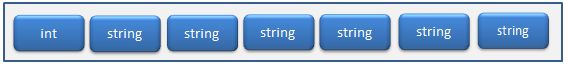
\includegraphics{expressionarray.png}
    \caption{Abstraction for the Expression Array. String refers to a string of integers}
\end{figure}


\subsection{Truevals Array}

The {\tt truevalsArray} stands for ``True Values" and it is generated in the Specific Ant XML file. The values to be passed into this array come from a function $f$. \\

 Let $f(A,B,S) = c$ be a function such that

\begin{itemize}
\item A is an input value from the Gene array (either T or F)
\item B is the factor value from the Expression array (an integer)
\item S is an external factor value coming from the Simulator, provided by the environment of the ant (an integer) 
\item c is the results in the computation of the fuction that represents the real value of the Gene type for the ant (an integer)
\end{itemize} 

This is shown in the following graph. See Figure 7: Abstraction for the Truevals Array

\newpage

\begin{center}
{\bf Generation of the Specific Ant XML}
\end{center}
 \vspace{-5 mm}
\begin{figure}[h!]
    \centering
    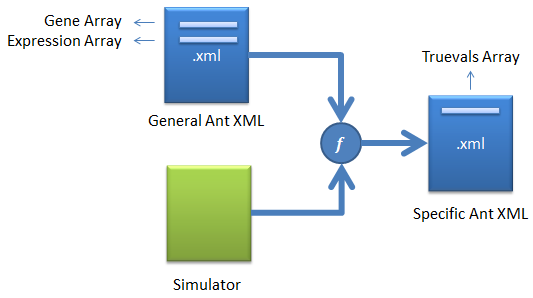
\includegraphics{specificchart.png}
    \caption{Abstraction for the Truevals Array.}
\end{figure}


The purpose of this True Values array is to provide the AI modules with information affected by the environment in the real world. \\

For instance, suppose that we want to characterize the behaviour of certain person. Suppose that person is usually very confident in itself, but is currently experiencing difficult times. Hence, the value of confidence of the person is actually less than his original (or normal) level of confidence. Likewise, we are trying to send information to the AI modules in which certain characteristics of the ant (genes) are modified or alter according to the current state of the ant and the nature of its environment. \\

The genes altered by external effects belong to a field called ``Epigenetics" which might be worth considering in a future in this project from a biology point of view. \\

Once $f$ is computed and stores the new values on {\tt truevalsArray}, then the method {\tt writeTruevalsArray} generates a new XML file which is the Specific Ant XML.\\

 This is the actual file that will be accessed by the higher modules of the ant brain to take actions and make decisions. The information inside the AI modules changes over time as it gets updated as it is executed. As a result, the ant's brain is saved in memory. 

\section{The Smell Module}
\subsection{Design of a better smell model}

In the previous section, we established ``Smell" as part of the DNA characteristic of the ant. In this section we explore a little more in detail the concept of ``Smell" and the importance of it. So far, in Prometheus, smell is represented by an integer value which is equal for all ants. The new model consists of adopting a more sophisticated version with the addition of multiple parameters. \\

The sensorial information collected by the virtual ants must have a parallel in the real world. Ants can detect pheromones traces and they also can spray them on the ground creating trails. The pheromone concentration is known to decay over time (in the order of minutes), and it must be constantly updated by the workers. \\

In addition to marking paths towards food with attractive pheromones, they use repellent pheromones to mark paths that should be avoided, for instance due to a depleted food source. As a result, trails can lose importance not only due to pheromone decay, but also due to explicit marking as suboptimal [2]. \\

In Prometheus, ants can smell and touch objects in their environment. It is possible to create new types of objects in the environment, each object has several attributes, such as decay, that simulate objects in real-life natural environment. As a result, the concept of Pheromone is abstracted in the following way: it is an object, with a speficif decay rate, a smell type that either attracts or repels the ant, a colony-specific type attribute, a name, etc. 
Each ant can create instances of this object. \\

A similar approach was chosen in this project. The virtual ant is able to deposit and sense different kinds of pheromones and odors. These have a dissipation rate and a dispersion rate. We will choose a level of abstraction which allows some creativity in our implementation.\\


\begin{center}
{\bf Smell Module}
\end{center}
 \vspace{-5 mm}
\begin{figure}[h!]
    \centering
    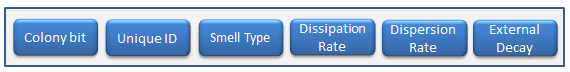
\includegraphics{smell.png}
    \caption{Abstraction for the elements of the Smell Module.}
\end{figure}
 
{\bf Elements of the Smell Module}
\begin{itemize}
		\item Colony Bit (an integer)
			\begin{itemize}
			\item Bit representing a type of colony. Different colonies have different bit 
			\end{itemize}
		\item Unique ID (integer string)
			\begin{itemize}
			\item Every ant not only carries its colony representation, but also its unique smell
			\end{itemize}
		\item Smell Type
			\begin{itemize}
			\item Repel or attract
			\item Efficient foraging: trail towards the shortest path to food or trail to avoid 
			\end{itemize}
		\item Dissipation Rate
			\begin{itemize}
			\item Rate at which ants spay the pheromones
			\end{itemize}
		\item Dispersion Rate
			\begin{itemize}
			\item Rate at which pheromone starts to fade out naturally due to lack of reinforcement
			\end{itemize}
		\item External Decay
			\begin{itemize}
			\item Humidity
			\item Water
			\item Wind speed
			\end{itemize}
\end{itemize}


%\section{Colony Simulation}
%Using ants in a simulated world that are guided mostly by smells and attempt to simulate the effects of learning memory, reasoning, modeling, conciousness, and more. We want to model: 
%\begin{itemize}
%\item How ants would work together in limited-constrained environments
%\item How two distinct colonies would interact with each other when there are limited food ressources
%\end{itemize}

%The 3D simulator attempts to emulate a real environment with terrain, water, sand, grass, and food. The ants can interpret this simulated world, and use their brain to perform tasks. The current brain controls the instinct of the ant, and uses information obtained from the environment to deduce actions. 

%To add: 
%\begin{itemize}
%\item We can use this simulator to apply predictive modelling to improve [something]
%\item The additional features include concepts that make the simulation more reaslistic and more efficient
%\end{itemize}

%\section{Ants and Neural Networks}

%Talk about the current version which includes implementing the Perceptron model and its current limitations. Mention that there is a better model which is the cascade correlation neural network\\

%According to some estimations, the entire nervous system of an ant comprises about 250,000 neurons. It is often mentioned that the ant is the creature with the largest neural system relative to its body size [3]. \\

%To add: 
%\begin{itemize}
%\item 1 individual ant behaves like a neuron in a single primate brain [J.Marshall, 2009]
%\end{itemize}

%\subsection{Perceptron Model}

%To add...

%\subsection{Cascade Correlation Neural Network}

%Introduce the concept of Cascade Correlation Neural Network and talk about this implementation can achieve better results

%To add: 
%\begin{itemize}
%\item KBCC is a child-learning process. The NN learns multiplication by incorporating previously-learned NNs such as addition and substraction.
%\end{itemize}

\section{Future work}

This project is a work in progress and is not yet completed. There are multiple implementations  under development. In a near future, the Specific Ant XML file will be successfully generated and implemented with the AI modules of the brain. In addition, the upgraded smell model will be tested and implemented in the Simulator. \\

Finally, we will use the Simulator to simulated world that are guided mostly by smells in which we will attempt to simulate the effects of learning memory, reasoning, modeling, consciousness, and more. We want to model: 
\begin{itemize}
\item How ants would work together in limited-constrained environments
\item How two distinct colonies would interact with each other when there are limited food resources
\end{itemize}

\section{Conclusion}
The goal of this project was to design and develop a database-like system for the Prometheus project. This was partially completed. In a near future, it is hoped that the AI modules will be able to incorporate the Specific Ant XML file. The importance of this project is that the virtual ant's brain is saved and it provides a framework to work with different ants avatars to simulate different environments and learning experiences which allows to get closer to the main goal of developing a brain for a fully autonomous robot. 

\newpage

%----------------------------------------------------------------------------------------
%	REFERENCE LIST
%----------------------------------------------------------------------------------------
\begin{thebibliography}{9}

\bibitem{lamport94}
  Robinson, E, Ratnieks, F \& M. Holcombe, 
  ``An agent-based model to investigate the roles of attractive and repellent pheromones in ant decision making during foraging". \emph{Journal of Theoretical Biology}, Volume 255, Issue 2, November 2008, p.250-258.
  
\bibitem{lamport94}
Ants. Oracle's ThinkQuest Library. {\tt http://library.thinkquest.org/} Retrived on August 2013. 

\bibitem{lamport94}
Julivert, A. \emph{The fascinating World of Ants}, Barron's Educational Series, 1991

\bibitem{lamport94}
Evison S.E.F, Beckerman, A.P, Ratnieks, F. ``Combined use of pheromone trails and visual landmarks by the common garden ant Lasius niger." \emph{Behavioural Ecology and Sociobiology}, Volume 63, 2008, p261-267.

\bibitem{lamport94}
Beshay, S, Shen, J. ``Prometheus Project: Ant Modeling and Inheritance". \emph{ECSE 476: Design Project I}, 2010

\end{thebibliography}




\end{document}
